\documentclass[dvipdfmx,uplatex]{jsarticle}
\title{知識と情報科学第1,2,3回}
\author{
    名前: 長田悠生\\
    学籍番号: 202310330\\
}
\date{2023/6/13}

\usepackage{url}
\usepackage{setspace}
\usepackage[dvipdfmx]{graphicx}

\begin{document}
  \begin{titlepage}
    \maketitle
    \begin{center}
      \textmc{\HUGE \LaTeX}
    \end{center}
    \thispagestyle{empty}
  \end{titlepage}

  \vspace{7mm}
  \textmc{\LARGE 第1回の要約\\}
  \textmc{
    \\
    第1回の講義では、様々な事象をどのようにコンピュータに解かせるのかについて掘り下げていた。
    話題は、プログラミングから始まる。プログラミングの特徴として、曖昧な支持ができないこと・目的に応じた時間に終わるの2ツつを挙げていた。次に、話題はアルゴリズムへと移る。
    まず、アルゴリズムそのものの説明が始まった。この講義では、アルゴリズムについて「問題を解決するための手順を定式化したもの」と説明されていた。入力されたデータをアルゴリズムによって、
    有限の手順で表現し、出力結果を導く。これがアルゴリズムの役割である。また、数学的な事象を扱うアルゴリズムを数理アルゴリズムと呼ぶそうだ。数理アルゴリズムの例として、物理シミュレーションと
    機械学習が挙げられている。この講義では、この2つの例についてさらに説明を加えていた。まず、物理シミュレーションについては、このように説明されていた。物理シミュレーションで扱う計算式は、
    支配方程式と呼ばれる諸島関数の組み合わせでは解くことが困難なものである。この支配方程式を効率よく計算できるようにアルゴリズムを考えるそうだ。次に、機械学習についてはこのように説明されていた。
    なお、この講義では教師有り学習の回帰と分類について説明している。説明の内容としては、複数の教師データをアルゴリズムによって、最も全体の誤差が小さくなるように仕組んである関数(モデル)に入れ、
    パラメータをアルゴリズムによって最適な状態に調整した後に、テストデータを入れてその精度を確認するというものだった。講義の終盤には、並列計算の話題にも触れていた。
    並列計算は、複数台のコンピュータで計算の高速化を図る者だが、並列計算向けのアルゴリズムの構築は難しいと述べられていた。\\
    }

  \vspace{7mm}
  \textmc{\LARGE 第2回の要約\\}
  \textmc{
    \\
    第2回の講義では、AIそのものについてと、AIに関するセキュリティについての説明だった。まず、AIについて説明する前に機械と人間の違いについて、得意・不得意の観点から説明されていた。
    機械が得意なことは、半永久的に消えない記録ができること、繰り返しの計算をし続けられることが挙げられていた。機械の不得意なこととしては、曖昧な情報の認識、直感的な判断、感情に関する
    情報の処理が挙げられていた。また、人間が得意とすることは、機械の不得意とすることとは対照的に、過去の知識を元に対称を一般化すること(汎化)が挙げられていた。
    しかし、AIは機会が苦手としている汎化というものができつつあり、シンギュラリティを迎える日も近いと説明されていた。そこから、話題はAIに関係するセキュリティの話題に移る。
    AIに関係するセキュリティの脆弱性の例として、敵対的サンプルとモデル反転を挙げていた。敵対的サンプルとは、画像や音声にノイズを混ぜて、AIに全く別の情報を意図的に認識させるように
    する攻撃手法である。また、モデル反転は、学習データを復元して攻撃を行うものである。この講義のまとめとして、「今後、攻撃するAIとその攻撃を防御するAI、防御するAIに守られるAIという関係ができるだろう。」
    と述べていた。\\
  }

  \vspace{7mm}
  \textmc{\LARGE 第3回の要約\\}
  \textmc {
    \\
    第3回の講義では、形状モデリングについての説明だった。形状モデリングとは、CGの分野において扱う対称の「形状」をコンピュータ内部のデータとして表現することである。
    この講義の主要な内容は、様々なモデルの表現方法である。まず1つ目に挙げていたのは、「点群モデル」である。点群モデルは、頂点座標だけを記録するために、立体の表現などが
    後処理なしでは難しいが、データ構造が単純なために、最近では自動運転等に利用されていると説明されていた。2つ目は「ワイヤーフレームモデル」である。ワイヤーフレームモデルは、
    データ表現が単純で計算が容易だが、裏側も見えてしまうために扱いにくく、形が一意に定まらない時があると説明されていた。3つ目は「ポリゴンモデル(三角形メッシュ)」である。
    ポリゴンモデルは、自然物などの数式では表現しにくい形状を扱いやすく、データ構造も単純であり、精度調整が容易なために、世界中でよく使われている表現手法であると説明されていた。
    4つ目は「ボリューム表現」である。ボリューム表現は、立体を3次元の格子状の小立体(ボクセル)の集合で表現するため、内部の構造を持て、データ構造も単純であるが、データ量が膨大で
    操作に時間がかかるという欠点があると説明されていた。また、この表現方法は、CTやMRIなどに利用されているとも言及されていた。5つ目は「パメトリック表現」である。パラメトリック表現は、
    区臆面上の座標x,y,zそれぞれを2変数(u,v)の関数で表すために、正確な形状定義ができ、微積分も容易であると説明されていた。6つ目は、「陰関数表現」である。陰関数表現は、F(x,y,z)=0となるような
    数式で表現される図形を表現するものであるために、正確な形状定義が可能であると説明されている。また、立体の内側$(<0)$と外側$(>0)$を定義できることにも言及されていた。
    7つ目は、「CSG表現」である。CSG表現は立体を基本立体と、その組み合わせで表現することができるので、データ量が少なく、立体の内部が詰まっているので、立体の内部と外部が定義できると
    説明されていた。最後に、「メタボール」について紹介していた。メタボールは、中心からの濃度で計算するモデルであると説明されていた。話題は、⽴体折紙の形状モデリングに移る。
    折り紙は、Developabilityという幾何学的な制約の下で成り立つ図形であり、具体的には、紙上に存在する直線の全ての交差点で$\sum \theta i = 2 \pi$が成り立たなければならない。
    その制約の下では、球を作ることは困難なので、しわを利用することで作成するのが可能なのではないのかという考えのもとで作成に挑戦されたお話をされていた。\\
  }

  \vspace{7mm}
  \textmc{\LARGE 第1回の講義についてのキーワード①: 物理シミュレーション\\}
  \textmc {
    \\
    私が高校時代に行っていたOpenFOAMを用いた流体シミュレーションについての説明をさせていただこうと思います。私は、高校2年から3年にかけてOpenFOAMを用いた流体シミュレーションに挑戦していました。
    シミュレーションの対象は、変形菌と呼ばれる生き物の子実体でした。1年間かけて何度もシミュレーションを行いましたが、2~3回程度しか成功せず、とても難しかった記憶があります。
    シミュレーションに用いた計算機は、高度情報科学技術研究機構(RIST)に貸していただいたマシンを利用しました。一度シミュレーションを体感しているので、今回の講義で出てきた物理シミュレーションについてのお話が
    とても身近に感じることができてうれしかったです。OpenFOAMの内部ファイルに書かれている関数の複雑さに、当時高校生だった自分は圧倒されていましたが、内部ファイルの計算効率が良いようにアルゴリズムが
    組まれていたのだと考えると、今更ながらとても感動しています。高校時代に作成した流体シミュレーションの半自動化システムについてまとめたウェブサイトを当時作成していましたので、以下にリンクを貼っておきたいと思います。
    また、作成したシステムの概要について簡単にまとめた動画もYouTubeにアップしていましたので、そちらのリンクも貼っときたいと思います。詳細について書くと、ページ数がオーバーしそうなので、
    私の作成したシステムに興味を持っていただいたら、ぜひウェブサイトと動画の視聴をしていただけるととてもうれしいです。\\
  }
  \textmc{\LARGE 第1回の講義についてのキーワード②: 機械学習\\}
  \textmc {
    \\
    1つの講義当たり1つのキーワードにしなければいけないですが、どうしても機械学習について書きたいことがあったので書かせていただきます。高校時代にすみれの葉の形態解析を、教師なし学習の一種である
    主成分分析で行っていました。講義中に出てきた、線形の次数下げの方法の1つの最小二乗法はとても懐かしい響きに感じました。主成分分析は、多次元ベクトルを2~3次元のベクトルに落として結果を表示する
    手法です。私は、高校時代にすみれの葉の長さをいろんな方向から測り、計6ベクトルのデータをcsvファイルに書き込んでR言語で計算させていました。最終的には、主成分分析のアプリ化に成功しました。
    以下に、主成分分析について自分でまとめたウェブサイトのリンクと、主成分分析のサンプルアプリ、実際に実装したアプリのリンクを貼っておきます。\\
  }
  \begin{figure}[h]
    \begin{center}
      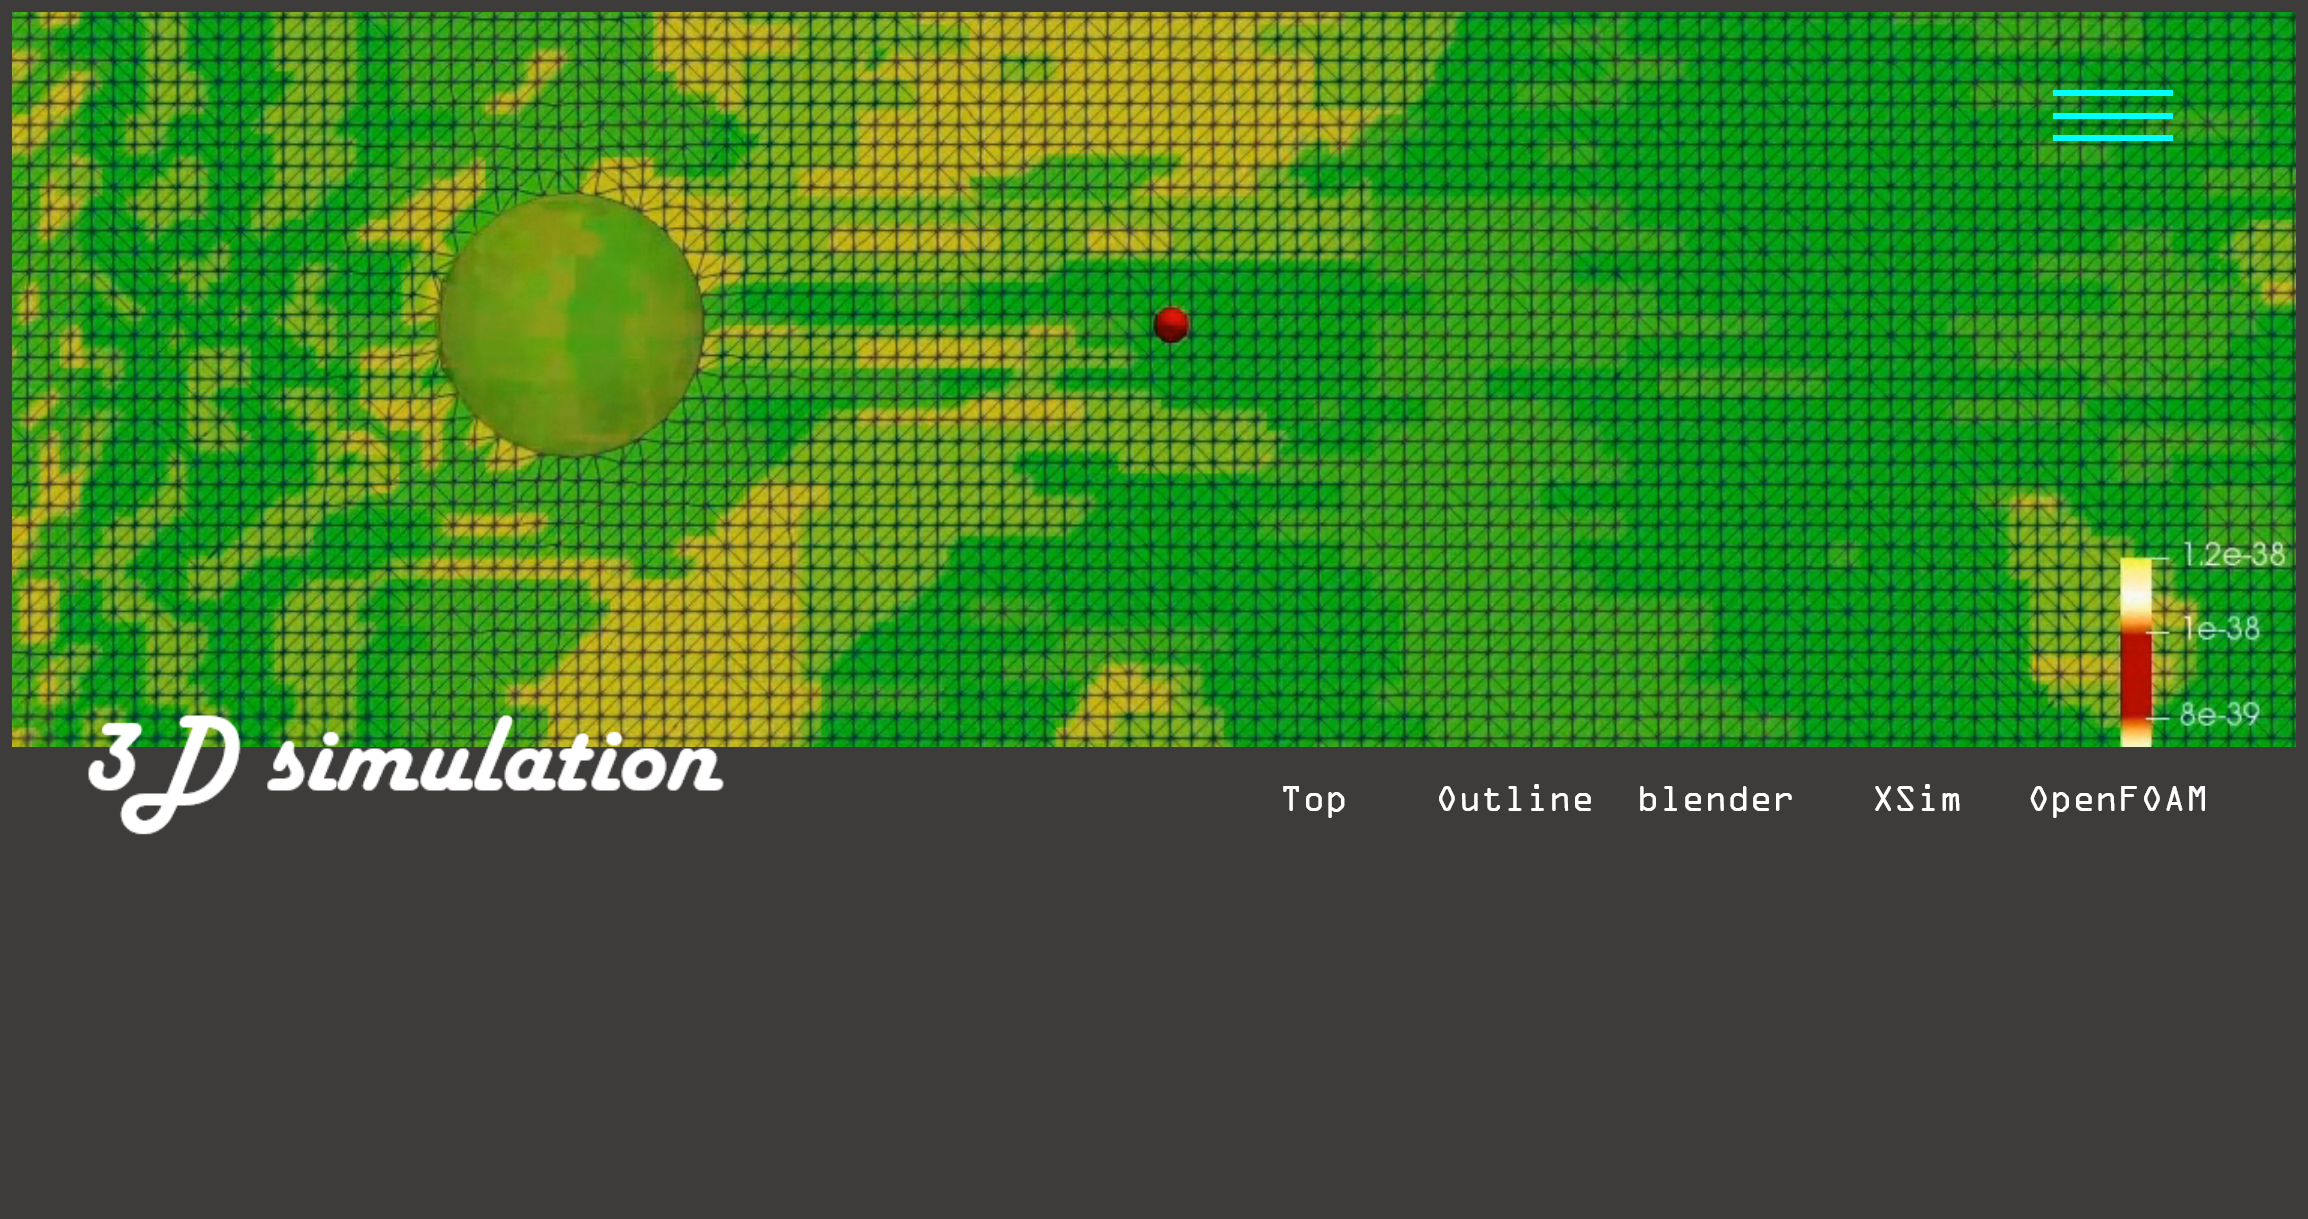
\includegraphics[width=100mm]{BSSO.png}
      \caption{自作したシミュレーションの半自動化システム}
    \end{center}
  \end{figure}
  \begin{spacing}{1.4}
    \centerline{\large 自作したシミュレーションの半自動化システム\\}
    \centerline{(OpenFOAMの環境構築の自動化が主なシステムの昨日となっています。)\\}
  \end{spacing}
  \centerline{\url{https://myxogastria0808.github.io/BSSO/}}
  \textmc{トップページのシミュレーションの映像は、実際に私が設定ファイルを作成して計算させたものです。\\}
  \begin{spacing}{1.4}
    \centerline{\large 自作したシミュレーションの半自動化システムの紹介動画\\}
    \centerline{\url{https://www.youtube.com/watch?v=n4zT5GOVXco}}
  \end{spacing}
  \begin{spacing}{1.4}
    \centerline{\large 主成分分析のサンプルアプリ\\}
    \centerline{\url{https://pcaplot.shinyapps.io/irisPCA/}}
  \end{spacing}
  \begin{spacing}{1.4}
    \centerline{\large 実際に実装したアプリ\\}
    \centerline{\url{https://myxogastria0808.github.io/PCA_App/}}
  \end{spacing}

  \begin{spacing}{1.2}
    \textmc{\LARGE 第2回の講義についてのキーワード: AIに対する攻撃手法\\}
  \end{spacing}
  \textmc {
    AIに対する攻撃手法には、データ汚染・モデル汚染・敵対的サンプル・データ窃取・モデル窃取の5つがあるようです。
    それぞれの攻撃手法における代表例を示していきます。まず、データ汚染ですが、"AIにバックドアを設置する手法"であるConvex Polytope Attackというのがあります。
    モデル汚染ですが、"AIの誤分類を引き起こす敵対的サンプル(Adversarial Examples)を作成する手法"であるFGSMというものがあります。敵対的サンプルですが、
    "AIによる物体検知を回避する手法"であるAdversarial Patchesというものがあります。データ窃取ですが、"AIの学習データを窃取する手法"であるMembership Inference Attacks
    というものがあります。モデル窃取ですが、"モデルを窃取する手法"であるCopycat CNNというものがあります。簡単にAIに対する攻撃手法について書いてみました。\\
  }
  \textmc {\small ダブルクオーテーションで囲んでいる部分は、下記に記載している参考文献の記事の引用になります。\\
    \\
  }
  \textmc{\LARGE 第3回の講義についてのキーワード: モデリング\\}
  \textmc {
    \\
    高校時代に、blenderでCGアニメーションを作成していたことがあるのでポリゴンメッシュのオブジェクトの作成は行ったことがあります。この講義を聞いていると、毛がふさふさになるテクスチャを貼ったりと、
    当時行っていたモデリング作業が思い起こされました。第1回についてのキーワードの部分で述べている流体シミュレーションの対象のオブジェクトもblenderで作成していました。blenderでモデリングをしていた時に
    一番驚いたのが、BlenderGISです。このプラグインは、マップの指定個所を切り抜くと町が立体に起こされます。また、一部のインフラの線もワイヤーフレームモデルで表現されており、初めて使用した時の感動は今も忘れません。
    モデリングやCGに関してまとめたサイトを作っていたので、以下にリンクを貼っておきます。\\
  }
  \begin{spacing}{1.4}
    \centerline{\large モデリングやCGに関してまとめたサイト\\}
    \centerline{\url{https://myxogastria0808.github.io/CG-Animation/}}
  \end{spacing}

  \begin{thebibliography}{99}
    \bibitem{総務省とMBSD}詳細解説 AIに対する攻撃手法と防御手法を解説します。, \url{https://www.mbsd.jp/aisec_portal/detail_attack.html} \\
  \end{thebibliography}

\end{document}